\cleardoublepage
\chapter{Design}
\label{ch:design}

\section{Design aims}

The design of Multiparty SessionJava (MPSJ) required taking into consideration different aspects of software engineering. The objective of providing a framework that can be easily utilised by the end-user often contrasted with the current implementation of SJ. The introduction of new methods and multiparty session types, referred to as \textit{global types}, created design considerations in terms of which calls should be left to the programmer vs. which methods can be implicitly called in the background and abstracted away from the user. 

In summary, the following list provides the main design aims developed in the initial stage of the project:

\begin{itemize}
\item Safe and type-checked structured interaction tools for multiparty sessions
\item Simple syntax for global types and general ease of programming
\item Overall efficiency and fast speed of interactions
\item Efficient integration into existing SJ code base, whilst mainting current functionality
\end{itemize}

The following design solutions are aiming at fulfilling the specified objectives in the best possible way. Their discussion involves justifications of any trade offs made as well as  


\section{Syntax}
\label{sec:syntaxdesign}

\subsection{Global Protocol Declarations}
\label{subsec:globprotdecl}

\paragraph*{Declaration Placing}
The idea behind SJ is to make collaborative network programming structured and safe through an initial agreement on a protocol, followed by programming the individual parts of the programs in accordance to it. MPSJ builds upon this idea by supporting protocol declarations placed as \textit{class members} and \textit{local variables}, which is compatible with SJ. 

MPSJ also offers the novelty of specifying the global protocol \textit{outside the class body}. This design choice provides the opportunity to declare the global protocol in a seperate file and exchange the file easily between programmers in the team. 

\paragraph*{Declaration Syntax}
The syntax design considerations for the multiparty session types presented the options of following the syntax from \cite{multiparty_sess_types} or modifying the syntax used currently by SJ to provide the additional functionality needed. The main difference is the lack of an explicit receive operation in the multiparty-session type syntax, as  shown in \autoref{TBglobtypesynt}. This in stark contrast with the current implementation of SJ.

MPSJ follows a mixture of SJ syntax and multiparty session type syntax which is shown in \autoref{TBglobprotsynt} below.

\begin{table}[H]
\center
\caption{Global Protocol Declaration Syntax}
\begin{tabular}{|l|l|}
  \hline 
  Syntax				&	Description												\\
  \hline	 
  \LST{global_protocol} &	protocol declaration keyword 							\\
  \LST{\{...\}}			&	global session type delimiter							\\
  \LST{a, b, ...}		& 	participant names										\\
  \LST{.}				&	session operation join									\\
  \LST{|a,b|}			&	session operation prefix								\\
  \LST{|a,b|!<int>}		& 	participant \LST{a} sends \LST{int} to \LST{b}			\\
  \LST{|b,a|?(int)}		&	participant \LST{b} receives \LST{int} from \LST{a}		\\	  
  \hline
\end{tabular}
\label{TBglobprotsynt}
\end{table} 

The declaration \LST{global_protocol InteractionProtocol \{|a,b|!<int>. |b,c|!<int>. |a,b|?(int) \} } therefore implies that the interaction starts with participant \LST{a} sends an integer value to \LST{b}. Participant \LST{b} then sends an integer value to particpant \LST{c} and the interaction finishes with participant \LST{b} receiving an integer from participant \LST{c}. 

Note that this design of global protocols uses a sense of duality, as the last interaction in the above example could be rewritten to \LST{|b,a|!<int>} without changing its the structure of interactions. This has been provided for better integration and compatibility with SJ as well as more user freedom in the presentation of the protocols. It may be desired to represent some parts of the interactions from the receiving end especially in large protocols to maintain clarity and similarity to the desired process models. This could not always be achieved if MPSJ fully adhered to \cite{multiparty_sess_types}.

\subsection{Programming in Multi-Party SJ}

The following code fragment in \autoref{LSTglobprotimpl} illustrates a short example of interactions programmed according to the protocol specified above. Initially the protocol has to be initialised to a new protocol variable. The protocol specification acts as a class, hence the initiation follows the standard Java practice.

\begin{lstlisting}[basicstyle=\LISTINGSTYLE, numbers=left, caption={Interaction implementation of the protocol from \autoref{subsec:globprotdecl}}, label={LSTglobprotimpl}]
public class Interaction {
	public static void main (String[] args) throws SJIOException {		

		InteractionProtocol prot = new InteractionProtocol();
	
		prot.a.setLocal();
		prot.b.setRemote("computer1", 1050);
		prot.c.setRemote("computer2", 1100);

		prot.invite();		

		int x = prot.b.sendInt();
		int y = prot.b.receiveInt();
	}
}
\end{lstlisting}

The methods \LST{setLocal()} and \LST{setRemote(String remoteName, int port)} are used to assign roles to the participants. They are invoked on the protocol variable and the participant to which the role is to be assigned. \LST{invite()} can only be called by one of the participants and it is important for all the other participants to have their ports open for incoming connections. To create all necessary links between the participants the inviting party delegates further invitations to other parties. All further interactions are similar to those of SessionJava with the difference that they are invoked on the protocol variable and participant as in the initial \LST{set...()} calls.

For other parties, which are on the receiving end of the session initiation the code fragment differs in the session setup method. The parties on the receiving end have to make a call to \LST{acceptInvite()} to initiate the session. The call has to be made before the \LST{invite()} is made on the initialising end. This is to ensure that the incoming connection port is open and ready to receive the session initiation call.

\section{Compiler Design Modifications}

The syntax and program design discussed in the previous sections impose several modifications onto the compiler. The syntax modifications need to be reflected in the langauge-indpendent grammar, additional AST nodes are necessary. An intelligent design has to be used to utilise the global protocol and the participants as the centres of interaction.

\subsection{Extending the Parser Generator for Global Session Types}

To support the definition of global protocols, or global session types in technical terms, as local variables, class fields and additionally as objects outside the scope of any class the design required a Java construct which could serve as a common denominator for all these declarations. Defining the global protocol as a construct similar to a class would match the requirements, as a Java class can be defined both in place of a class member and locally in a method. 

Lexically, a class definition is identified as a type declaration. The parser generator was therefore extended to interpret a global protocol declaration as a type declaration. This enables the compiler to recognise any global protocol as a type with the ability to instantiate variables of this type as shown in line 4 of \autoref{LSTglobprotimpl}.

\begin{figure}[htb]
\begin{center}
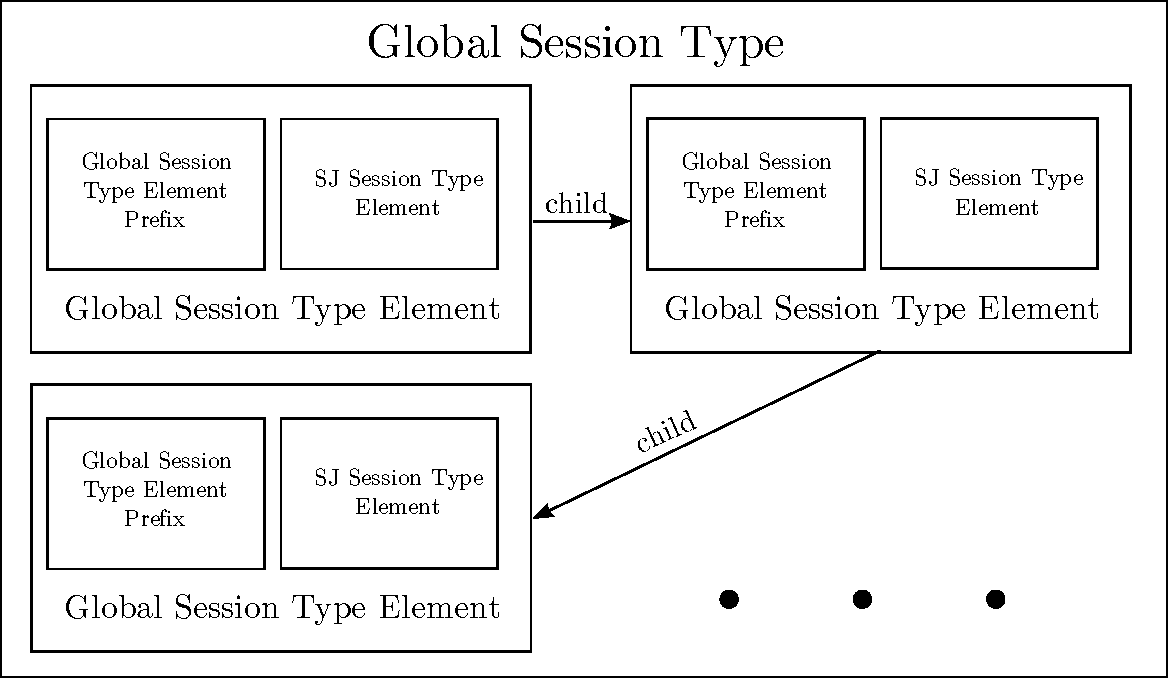
\includegraphics[width=0.8\textwidth]{globsesstypeelement}
\caption{Structure of a Global Session Type}
\label{fig:globsesstypelement}
\end{center}
\end{figure}

The parser generator also had to be extended to correctly recognise a global session operation of the structure \LST{|a,b|!<int>} of which a global session type consists. \autoref{fig:globsesstypelement} shows the structure of a \textit{global session type}. For a global session type to be valid, it has to have at least one \textit{global session type element}, which in turn consists of a \textit{global session type element prefix} and a standard \textit{SJ type element}. This construct together is interpreted as one global operation. Any number $n$ of subsequent operations can be defined as children of previous operations as in the figure. 

The discussed design permits MPSJ to use the SJ code efficiently as it follows similar patterns and provides enough flexibility for future extensions. The specific implementation of the syntax discussed in \autoref{subsec:ppgimpl} ensures safe permformance of lexical analysis so that the majority of structural mistakes can be recognised at the initial stages of the compilation process.


\subsection{Modifying the AST Node Structure}

As discussed in \autoref{subsec:polyglotarch} the generated parser calls relevant methods in the \textit{node factory} to generate the AST nodes that correspond the syntactic elements. Given the extensions specified above there is the need to create additional nodes in order to represent the additional parts of the syntax.

\LST{SJGlobElementPrefixNode} acts as the prefix and is constructed out of two \LST{Identifier} nodes which represent the participants. Together with an \LST{SJTypeNode} which depicts the operation the nodes form a \LST{SJGlobTypeNode}, which has a field \LST{child} of type \LST{SJGlobTypeNode} to encapsulate the next operation in the sequence.

Finally all the information about the session is enclosed in the \LST{SJGlobProtocolDecl} node with the addition of the protocol name in form of an \LST{Identifier} and any flags such as \LST{public} or \LST{private}. 

\subsection{Global Protocol as the Core of Interaction}

\autoref{sec:syntaxdesign} made it explicit that all interactions in MPSJ revolve around the global protocol. \autoref{fig:globprotocol} illustrates the design pattern used to achieve this. During the compilation process the global protocol is effectively transformed into a class with the participants as its members. In that way the global protocol becomes the session interaction centre. If methods such as \LST{invite()} or \LST{acceptInvite()} relate to the session as a whole, the operations are performed on the global protocol. Other methods concerning specific session participants such as \LST{send()} or \LST{receive()} are performed on the participant objects. Invoking  

\begin{figure}[htb]
\begin{center}

\includegraphics[width=0.8\textwidth]{globprotocol}
\caption{Global Session Interaction Points}
\label{fig:globprotocol}
\end{center}
\end{figure}



\section{Runtime Design Alterations}

\subsection{Use of Session Participants as SJSockets}

\subsection{Creating the Multi-Party Session}